\leadauthor{Bisot}
\title{Carbon supply for growth drives network-wide bidirectional flows in mycorrhizal fungi}

\shorttitle{Nutrient circulation in Mycorrhizal fungi}
\author[a,b,c,*]{Corentin Bisot}
\author[b,*]{Simon van Staalduine}
\author[b]{Achille Joliot}
\author[a,b]{Loreto Oyarte Galvez}
\author[d]{Filipe Henrique de Sousa Evangelista}
\author[a]{Marije van Son}
\author[d,f]{Howard A. Stone}
\author[a,e,f]{E. Toby Kiers}
\author[b,f]{Thomas S. Shimizu}

\affil[a]{Amsterdam Institute for Life and Environment, Vrije Universiteit, Amsterdam, The Netherlands}
\affil[b]{AMOLF Institute, Amsterdam, The Netherlands}
\affil[c]{European Molecular Biology Laboratory (EMBL), Heidelberg, Germany}
\affil[d]{Department of Mechanical and Aerospace Engineering, Princeton University, Princeton, NJ, United States of America}
\affil[e]{Society for the Protection of Underground Networks (SPUN), Dover, DE, United States of America}
\affil[*]{These authors contributed equally}
\affil[f]{co-corresponding authors}
\date{}
\maketitle

\begin{abstract}
 
Plant-mycorrhizal symbiosis is fundamental to terrestrial ecosystems as it is responsible for large flows of nutrients on a planetary scale.
In this symbiosis, two distinct organisms trade phosphorus (P) for energy in the form of carbon (C).
However, the mechanism behind the bidirectional transport of resources within their microscopic hyphae has not been entirely elucidated.
We imaged transport dynamics of nutrient flows in high resolution in different positions in growing networks, and also perturbed flows through segment cuts and osmotic shocks.
We find that carbon likely moves across the fungus on a directed network of molecular motor filaments.
Our findings also suggest a tight coupling between network growth, internal carbon (lipid) transport dynamics, and bidirectional fluid movement within the network.
The movement of lipids in the open pipe system inherently produces a backflow of cytoplasmic fluid, which may be responsible for the movement of phosphorus.
Our model provides an intuitive understanding for the observed proportionality in resource exchange between the two organisms.
% NOTE (15 Oct, main-text review): According to the C/P note in the Discussion, the model makes the returning volume proportional to the motor-carried carbon by construction (slope 1.000), but not to growth carbon (slope 0.19, 95 % CI -0.47 to 0.86, 15 sessions), so 'understanding of the observed proportionality' needs that qualifier. Also, the perturbations listed are segment cuts and osmotic shocks, and the root cut is missing.
\end{abstract}

\section*{Introduction}
\subsubsection*{Why bidirectional transport matters}
\paragraph*{A long-lived, many-to-many symbiosis needs mechanisms against free riders}
The symbiosis between Arbuscular Mycorrhizal (AM) fungi and their host plants has existed for 400 million years~\cite{remy_four_1994,brundrett_evolutionary_2018}.
For the symbiosis to endure this long, robust mechanisms must be in place to ensure its stability.
Indeed, symbiosis can be a many to many relationship, which means that the plant can interact with multiple independent fungal colonies and one fungal network can interact with multiple plant hosts~\cite{kiers_reciprocal_2011,walder_mycorrhizal_2012}.
Without selective orientation of nutrients towards partners that engage in a proportional effort to provide nutrients, "free ride" plant or fungal phenotypes can emerge that reap the benefits of symbiosis while avoiding costs~\cite{kiers_reciprocal_2011,bever_preferential_2009,walder_regulation_2015,noe_mycorrhizal_2018,kiers_misconceptions_2016}. 

\paragraph*{Carbon must reach the growing edge and phosphorus the root, through open pipes}
The fungal partner forms a network in the soil using plant derived carbon.
It absorbs phosphorus from the soil, which is then transported back to the plant.
This means that carbon must constantly be shipped to the growing edge of the colony away from the plant, while phosphorus needs to be transported back in the other direction.
Like other coenocytic fungi, AMF have aseptate hyphae, meaning that the organism can be considered a fully open pipe system, while they are growing.
The mechanisms that could explain such bidirectional transport in a network of open pipes are so far unknown.

\paragraph*{Phosphorus delivery is proportional to carbon received}
Our group had previously estimated that the fungal use of carbon for growth was proportional to the flux of phosphorus towards the plant~\cite{bisot_carbon-phosphorous_2025}, when a single AM fungus was attached to a single plant.
In addition, it has been observed in the past that, when a single AM network was connected to two different plant hosts that differed in their carbon supply, more phosphorus was directed towards the plant that provided more carbon~\cite{kiers_reciprocal_2011}. 

\subsubsection*{What is known about flows in AM fungi}
\paragraph*{Speeds are known in both directions, not which resource moves where}
Past research has quantified the flow speed in both directions in networks of different ages~\cite{oyarte_galvez_travelling-wave_2025}.
However, without staining the lipids and/or phosphorus, it is difficult to understand the organization of resource flow across the network and the underpinning transport mechanisms.
Resource specific staining can shed light on the distribution of resource flux within the network.
For example, using Nile Red staining and two-photon microscopy, it was found that lipid density varies along the hyphae, from about 24\% of the hyphal volume near the root to about 0.5\% at the front, and that lipid bodies move in both directions, mostly with the cytoplasmic stream~\cite{bago_translocation_2002}.
A role for microtubule tracks in this movement has been proposed, and microtubules have been imaged across the network~\cite{uetake_extensive_2002}, but to our knowledge the link between microtubules and lipid transport has never been established.

\paragraph*{Speeds correlate with betweenness centrality, without a mechanical basis}
Flow speeds along the hyphae are modulated with time and location within the network~\cite{oyarte_galvez_travelling-wave_2025}.
This can be interpreted through a traffic analogy inspired by the observed correlation between betweenness centrality, a typical transport network metric, and flow speeds.
The betweenness centrality being the sum of times a shortest path between arbitrary nodes in a network crosses a particular network edge.
Here, we set the root and tip nodes as the set of source and target nodes.
However, this correlation lacks a direct physical basis that explains how such a relationship between global metrics and flows could emerge mechanically.
Because AM fungi are coenocytic, the colony can be represented as a hydraulic network of connected pipes with varying radii.
This hydraulic coupling between all elements of the network could generate spatial correlation in ways that can be physically framed.
Such a mechanical framework, validated against measurements, for growing AM colonies is still missing.

\subsubsection*{Questions and approach}
What mechanisms explain the bidirectional transport of resources in the colony and its modulation over space and time?
How can the transport mechanisms in place maintain a form of bidirectional transport in which the magnitudes of resource flux in opposite directions are maintained proportional? 
To answer these questions, we acquired image data at two different spatial and temporal resolutions to quantify the flow speed in specific edges of growing networks.
At high spatial and temporal resolution, we acquired bright-field videos of transport dynamics within single hyphal edges over multiple days.
Using Nile red, a neutral lipid-specific fluorescent dye, we also characterized and quantified the movement of carbon in the form of lipids along these same edges.
At low spatial and temporal resolution, we obtained time-lapse images of growing networks that were transformed into their equivalent mathematical graph.
In this way, we can relate the growth of the network with the measured flow speeds observed in the same network, allowing us to explain high-resolution observations both mechanistically and quantitatively.
Additionally, a small number of perturbation experiments were performed to characterize each flow direction.
From these data and findings, we construct a minimal model that explains the observed bidirectional transport of resources in the colony and its modulation over space and time.

\section*{Results}
\namedsubsection{Asymmetric bidirectional speeds}{subsec:res_speeds}
\subsubsection*{Topological context changes along a hypha}
Fungal networks grow through the extension of fungal tips away from the root of the host plant.
Over time, these elongated hyphae develop into a branched mycelial structure.
The network's topological context therefore varies along the length of a hypha.
Close to a growing tip, the network is more tree-like: 40\% of the edges within 1~mm of a tip are bridges, that is, not part of any loop, versus 11--14\% of the edges further than 2~mm from a tip (Fig.~\ref{fig:hyphal_profiling}A, inset).
Moving away from the tip, more growing hyphae depend on the same runner hypha, and anastomosis (fusion between a hyphal tip and a hyphal segment) creates loops, which give many alternative paths from the tip towards the root~\cite{oyarte_galvez_travelling-wave_2025}.

\begin{figure}
    \centering
    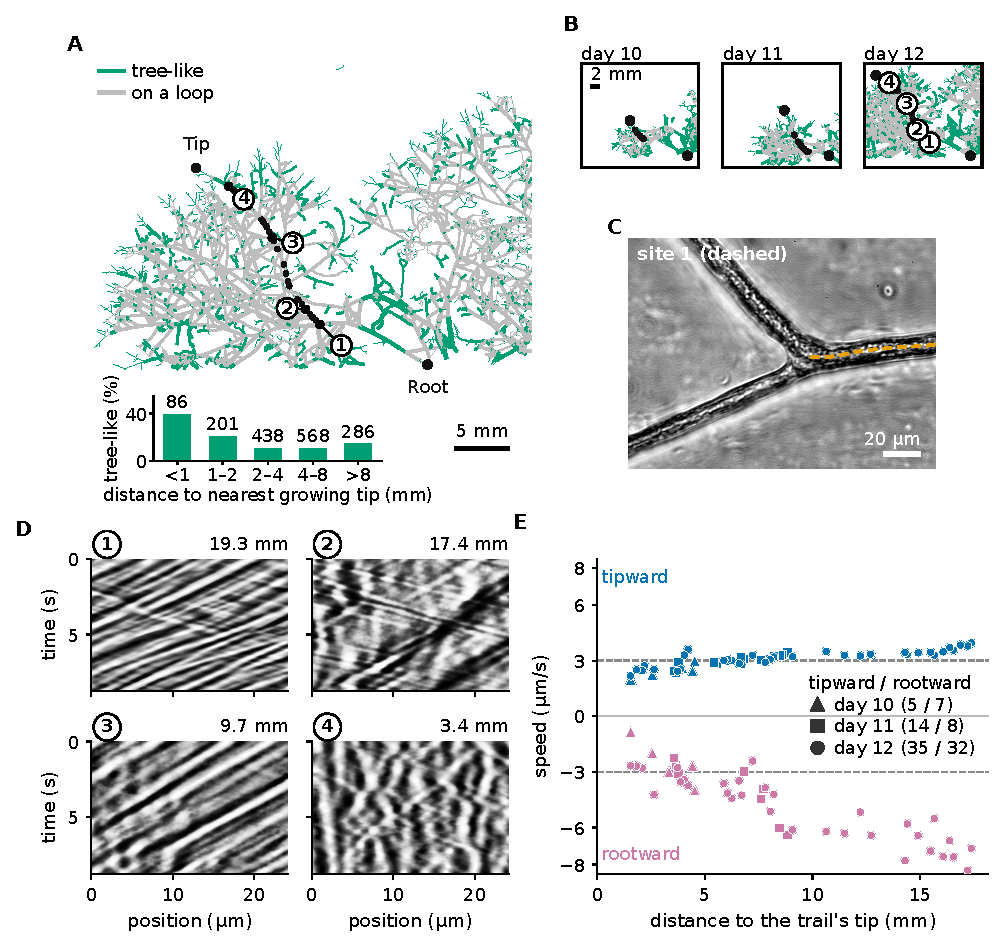
\includegraphics[width=\textwidth,height=0.72\textheight,keepaspectratio]{figures/Figure_1_v4.pdf} 
    \caption{\textbf{AMF produce robust patterns of asymmetric bi-directional flows across time and space.}
\textbf{(A)} Network graph where a hyphal transect has been highlighted with dots where measurements took place.
Green edges are tree-like, grey edges lie on a loop; line weight is exaggerated hyphal diameter.
Inset: share of tree-like edges among the filmed edges (15 networks) by network distance to the nearest growing tip; numbers are edges per bin (SI, \nameref{subsec:si_tree_tip}).
\textbf{(B)} Time evolution of network across three days after the network started crossing into the fungal compartment.
Dots indicate locations where videos were taken.
\textbf{(C)} Example video frame of site 1, with edge indicated which is shown in D1.
\textbf{(D1, 2, 3, 4)} Kymographs from respective locations in B, normalized by time-averaged value, and enhanced with CLAHE~\cite{pizerAdaptiveHistogramEqualization1987}.
\textbf{(E)} Velocity profile along the trail shown in A, relative to the distance from the tip at the time of measurement.
Each point is one video: the median of its extracted tipward (blue) or rootward (pink) speeds.
Marker shape gives the day, with the number of videos tipward / rootward in the key; dashed lines mark $\pm 3~\mu m/s$.}\label{fig:hyphal_profiling}
\end{figure}

\subsubsection*{Tipward and rootward speeds along runner hyphae}
\paragraph*{Flows filmed on runner hyphae of five colonies, in bright-field and Nile Red}
We asked how this change in topological context affected the speeds of the flows in the two directions along a hypha: towards the growing tip (tipward) and towards the root (rootward), as defined by the growth direction of the network.
We imaged flows at high resolution in 731 bright-field videos along the hyphae of five colonies (SI Fig.~\ref{fig:video_positions}) and, mostly at the same positions, in 625 videos of Nile Red fluorescence; for the example network of Fig.~\ref{fig:hyphal_profiling}, the videos were taken over three consecutive days.
We chose runner hyphae, the main routes to the root and the edges of high betweenness centrality~\cite{kirkley_betweenness_2018}, where the tipward and rootward flows could be told apart by eye (SI, \nameref{subsec:si_video_selection}; SI Fig.~\ref{fig:bc_selection}). 

\paragraph*{Tipward speeds stay near 3~$\mu m/s$, rootward speeds rise with tip distance and vary more}
In undisturbed hyphae (SI, \nameref{subsec:si_lid}), the two flows are superimposed in the video and move in straight lines at nearly constant speed, so that in a kymograph every moving particle leaves a straight diagonal streak, with no sign of random or back-and-forth movement, except near the tips (Fig.~\ref{fig:hyphal_profiling}D).
In the field of view, the directed movement exceeds diffusion by more than two orders of magnitude, so the slope of a streak is its speed.
% NOTE (6 Oct, answers Coco's 'why is there little diffusive movement?'): This is a Peclet estimate, to order of magnitude only. It assumes a lipid droplet of 0.5 um diameter, a cytoplasm viscosity 10 times that of water (0.01 Pa s) and T = 295 K, which give D = kT/(6 pi eta r) = 0.09 um^2/s. Over a 10 s kymograph, diffusion covers sqrt(2Dt) = 1.3 um, against 30 um of transport at 3 um/s. With L = 10 um, Pe = vL/D = 350. Check the droplet size and viscosity before submission. The argument is weaker near the tips (Fig 1D kymograph 4); see issue #5.
Each streak gives one speed, and each kymograph was reduced to a set of tipward and rootward speeds (SI Fig.~\ref{fig:speed_flux_extraction_real_data}).
In the histogram of the extracted speeds of a video, the tipward speeds (positive) and the rootward speeds (negative) each form a peak.
We took the median of each of the two groups as the speed of that direction in that video (Fig.~\ref{fig:hyphal_profiling}E). 
The tipward speeds slow down near the tip, but stay close to 3~$\mu m / s$ further away (Fig.~\ref{fig:hyphal_profiling}E).
Rootward speeds generally increase with distance from the tip (Fig.~\ref{fig:hyphal_profiling}E), and have a wide range: the median interquartile range of a hypha's speeds is 1.6~$\mu m / s$ rootward, against 0.6~$\mu m / s$ tipward (SI Fig.~\ref{fig:speed_iqr}).
This result was confirmed by repeating a similar experiment on various plates over 15 repetitions over 5 plates showing a consistent phenomenology (Fig.~\ref{fig:asymmetries} A, B). 
% NOTE (15 Oct, main-text review): '15 repetitions over 5 plates' means 15 sessions on 5 plates.

\begin{figure}
 \centering
 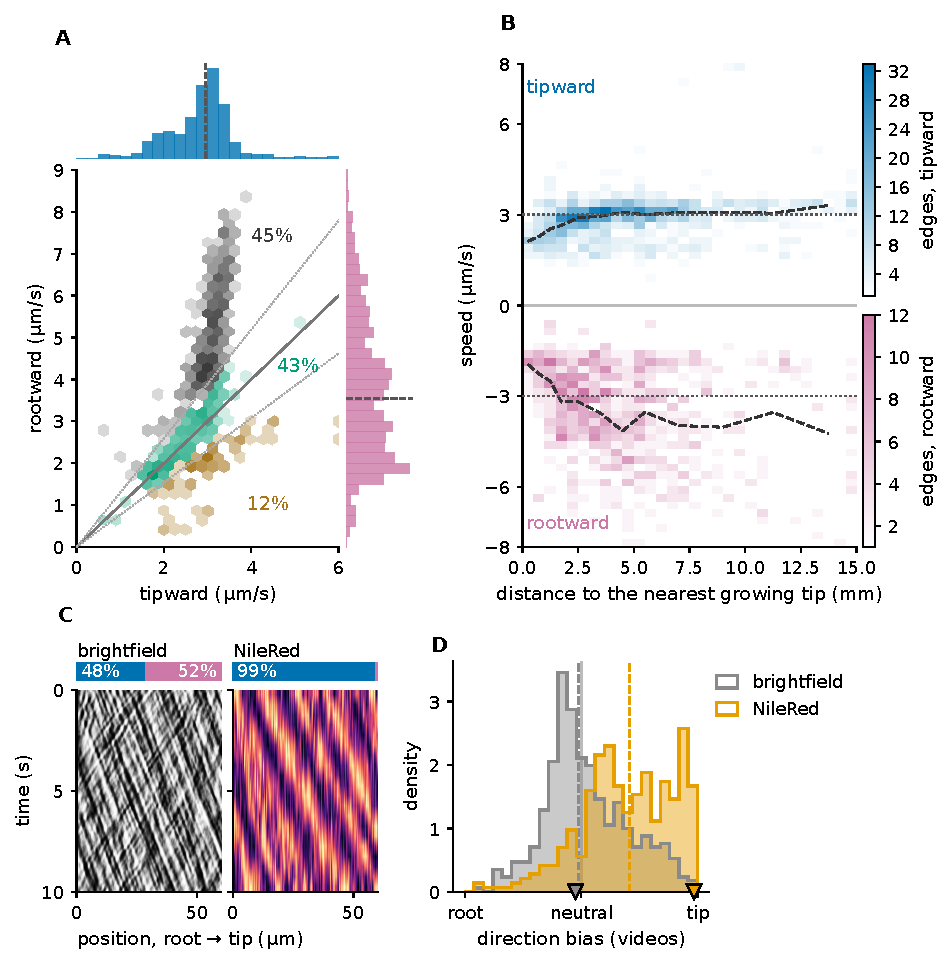
\includegraphics[width=\textwidth]{figures/Figure_2_v2.pdf}
 \caption{\textbf{Tipward and rootward flows differ in speed and in cargo: the tipward flow is concentrated around $3 ~\mu m /s$ and carries most of the lipid, the rootward flow is more variable.}
\textbf{(A)} Density of the absolute tipward speed against the absolute rootward speed at the same location, in bright-field.
Marginal histograms along the edges.
Hexagons are coloured by their ratio to 1:1 within a factor 1.3: rootward faster (black), similar (green) or tipward faster (orange); percentages give the share of the data in each class.
\textbf{(B)} Density of the measured speeds against the distance to the nearest growing tip: tipward (blue) and rootward (pink), with the median per column (dashed) and $\pm 3 ~\mu m/s$ (dotted).
\textbf{(C)} The same position imaged in bright-field (left) and Nile Red fluorescence (right), 15 seconds apart; bars give the share of the speed-weighted moving signal going to the tip (blue) and to the root (pink).
\textbf{(D)} Direction bias per video, the share of the speed-weighted moving signal going to the tip (median over the edges of the video; videos with too little directed signal left out), from bright-field (grey) and Nile Red fluorescence (yellow, median .71).
Dashed lines: medians; triangles: the example shown in C.}\label{fig:asymmetries}
\end{figure}
% NOTE (16 Oct): The fluorescence speed sentences of the next subsection (lipids at 2.42 against 2.95 um/s; 989 against 1,396 rootward streams at 2.20 against 2.91 um/s; the video and edge counts in the bias paragraph) compare fluorescence and bright-field speeds, which Simon decided to drop on 13 Oct (detection limit; the SI comparisons are out). The direction bias (Fig 2D) does not depend on speeds and stays.

\subsubsection*{The lipid cargo moves mostly to the tip}
\paragraph*{Lipids move to the tip at the bright-field tipward speed; fewer, slower lipid streams go to the root}
We asked if the asymmetry in the directional speeds could be due to the difference in cell components that would be moving in the two directions, which could inform the mechanism of movement.
We stained neutral lipids with Nile Red fluorescent dye~\cite{bago_tracking_2002} and imaged the same positions with both bright-field and fluorescence setups (Fig.~\ref{fig:asymmetries}C, D).
At the resolution of the fluorescence videos (0.14~$\mu$m per pixel, 0.5 or 1~s per frame, 10 to 20~s per video), we saw no evidence of lipid particles randomly switching direction, as they would in the random walk underlying diffusive motion (Fig.~\ref{fig:asymmetries}C).
The lipids moved to the tip at a median of 2.42~$\mu m/s$ (879 edges with both directions measured in fluorescence), insignificantly different from the 2.95~$\mu m/s$ of the bright-field tipward stream.
In the other direction, fewer fluorescence streams were detected (989 against 1,396 tipward), at a median of 2.20~$\mu m/s$ against 2.91~$\mu m/s$ in bright-field.

\paragraph*{Lipids have a tipward direction bias of 0.71, bright-field is roughly even}
By comparing bright-field and fluorescence videos of the same position, recorded about 15 seconds apart, it is clear that only a subset of trails visible in bright-field kymographs appear also in the fluorescence version (Fig.~\ref{fig:asymmetries}C, D): fluorescence gives 625 videos and 879 edges with both directions measured, bright-field 731 videos and 1,513 edges.
We set out to find whether there was a directional bias in the movement of lipids.
For each video we computed the share of the moving signal that travels towards the tip, from 0 (all to the root) to 1 (all to the tip) (Methods, \nameref{subsec:direction_bias}).
Together, these results show that lipids generally move in the direction of the tips (Fig.~\ref{fig:asymmetries}D): we found a median direction bias of 0.71 towards the tips, with 84\% of edges having lipids with a tipward direction bias, against roughly even for brightfield in both metrics. 

\namedsubsection{Perturbations show that cytoplasmic flow toward the root is pressure driven while tipward flows are likely locally driven and pressure-insensitive}{subsec:res_perturbations}
\begin{figure} 
\centering
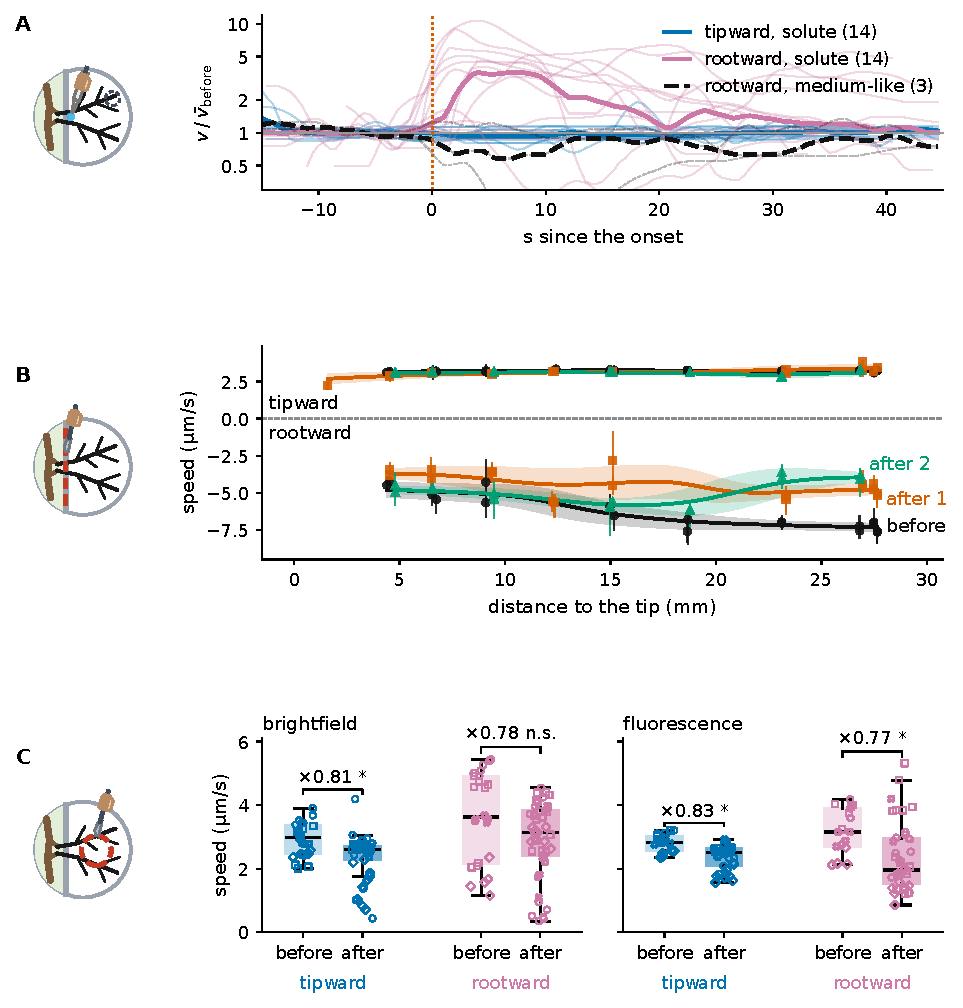
\includegraphics[width=\textwidth]{figures/Figure_3_v3.pdf} 
\caption{\textbf{Flows are driven by local elements, with limited whole-network influence.}
\textbf{(A)} Osmotic shock: a drop of solute solution (mostly NaCl, 50 to 400 mOsm) placed on the substrate at the base of the network, a few centimeters behind the growing front, while a hypha near the growth edge is imaged.
Speed divided by its mean before the drop, tipward (blue) and rootward (pink): thin lines are single droplets, thick lines the median of the 14 solute droplets; the black dashed line is the median rootward speed of 3 medium-like control drops.
Dotted line: onset of the response.
\textbf{(B)} Root cut: the network is severed from the root along its whole bottom.
Speed along a runner hypha against the distance to the tip, 5 min before (black), 5 min after (orange) and 30 min after (green) the cut.
Positive speeds are tipward, negative rootward.
Points are positions along the hypha (bars: interquartile range of the videos), curves the kernel-averaged mean and shading $\pm 1$ standard deviation.
Time windows when videos were made are 15:19--15:40 (before), 16:01--16:17 and 16:37--16:51 (after).
\textbf{(C)} Section cut: a sub-graph of the network is isolated by cutting its connections (red lines in the icon).
Speed before and after the cut in bright-field and in Nile Red fluorescence, tipward (blue, positive) and rootward (pink, negative).
Each dot shape is one isolation cut video. Significance of the posterior median ratio after/before is indicated by stars: P (direction) >= 0.95 *.
Pre-cut data were acquired up to 40 minutes before the cut, post-cut data from 4 minutes to 2 hours after.}\label{fig:perturbations}
\end{figure}

\subsubsection*{Diffusion, mass flow and peristalsis do not explain two opposing steady streams}
In the past, pressure gradients and molecular motors have been suggested to be potential mechanisms driving flows in fungal hyphae~\cite{steinberg_cell_2017,kokkoris_mycelial_2026}. 
It is also important to discuss other potential mechanisms that could drive flows in fungal hyphae, and to evaluate whether our data support or contradict each of them. 
Diffusion as a mechanism could be present close to the tips, as that is where we observe the most random movement of particles (Fig.~\ref{fig:hyphal_profiling}D4), but the directed, unbroken flow in the rest of the network is not consistent with diffusion alone. 
Singular mass flow, as suggested by previous work~\cite{heaton_growth-induced_2010,lew_mass_2005,lew_how_2011}, is also unlikely to be the main driver of flows in our system, as it cannot explain the presence of two opposing streams at similar speeds in the same hypha (SI, \nameref{subsec:si_mass_flow}). 
Peristaltic flow has been observed and studied in \textit{Physarum}~\cite{alim_mechanism_2017}, but involves flow reversals that are not observed in our system when atmospheric pressure and moisture are kept constant (SI, \nameref{subsec:si_lid}). 

\subsubsection*{Perturbations separate the two directions}
\paragraph*{An osmotic shock raises the rootward speed briefly and leaves the tipward speed unchanged}
The difference in flow behavior both within an edge and along an edge with distance to tip suggests that each direction could be associated with a different mechanism.
An ideal experiment to distinguish these two potential drivers would be to modify the pressure gradient across the network and see how it affects flows.
This experiment has been performed in the past by creating an extracellular osmotic gradient~\cite{lew_mass_2005}.
Following a similar approach, we added a drop of dissolved either NaCl or sucrose solution (50 to 400 mOsm) (Methods, \nameref{subsec:perturbations}) to the base of the network a few centimeters behind the growing front and imaged near the growth edge (Fig.~\ref{fig:perturbations}A).
We expected that this would create a low turgor pressure within the hyphae at the location of the drop, shifting the pressure gradient within the network, and therefore changing flows internal to the hyphae.
We observed that the flow speed in the tip direction was almost unaffected by the addition of the salt solution  (Fig.~\ref{fig:perturbations}A);  fluorescence imaging of the lipids showed that their movement in the tip direction was also unaffected (SI Fig.~\ref{fig:salt_shock}D).
By contrast, the flow speed in the root direction was approximately increased to 3.5 times and relaxed in a minute.
Medium-like drops resulted in what looked like light hypo-osmotic shocks, pushing the flow towards the tips.

\paragraph*{After a root cut both flows continue: the plant connection is not needed}
Past work proposed that plant host transpiration could be the driving force explaining the flow of resources towards the root~\cite{kikuchi_aquaporin-mediated_2016}.
Although the plant in our root-organ culture does not produce leaves and, therefore, does not evapotranspirate, we wanted to test whether the connection to the plant was necessary for the flows in the two directions to be maintained.
In one network, we imaged a runner hypha at multiple positions from root to tip to measure the velocity profile along its length.
We then severed the network from the root with a scalpel cut along its entire bottom (Fig.~\ref{fig:perturbations}B) and recorded the same positions again, in the first half hour after the cut, and then again in the second half hour.
Flows continued in both directions.
The tipward speed remained at about 3~$\mu m/s$, and the rootward speed decreased and became flatter along the hypha, but the asymmetry between the two directions remained (Fig.~\ref{fig:perturbations}B).
This matches earlier work showing that flows can still be active a year without a plant host~\cite{kleinCytoplasmicFlowDynamics2026}.
A connection to the root is therefore not needed for either flow, which rules out transpiration by the plant as their driver.
How far a driving force can reach is a separate question, and we asked it by further shrinking the connected network.

\paragraph*{In isolated segments of a few millimeters both flows continue, about a fifth slower}
To further hone down on the range of a potential driving force, we wanted to know what the minimal size of the subgraph was that was necessary to conserve flows in the two directions.
We made targeted cuts to isolate small segments from the network and image flows at sufficient distance from the cut induced stress (Fig.~\ref{fig:perturbations}C).
In patches of network as small as only a few millimeters in total length, we still observed flows in the two directions (Fig.~\ref{fig:perturbations}C).
We observed that the flow speed of the lipids in both directions was affected, slowing down about 20\%, but the flow never stopped (Fig.~\ref{fig:perturbations}C).
In none of the experiments did the flow stop.
These experiments demonstrate that the mechanical origin of flows in the two directions does not require long range connectivity of the network to operate (SI, \nameref{subsec:si_segment_size}). 
% NOTE (15 Oct, Simon): The repeated isolated-segment paragraph in the single-pipe section ('An isolated segment keeps bidirectional flow, as the model predicts') was removed. Three pieces of it may be worth reusing here: the model's prediction that a pipe closed at both ends (net water flux zero, small lipid fraction) keeps a return at about v0 (eq. max_speed); the clotting after cutting, with the gellin precedent (nguyen_fungal_2021); and the link to SI video 3 (https://www.dropbox.com/scl/fi/ors0lqpopi5yymh6e79o9/SIvideo3.avi). Its claim that both speeds stay close to 3 um/s did not match Fig 3C, where both streams are about a fifth slower.

\namedsubsection{Our hypothesis on the flow mechanics, given the evidence}{subsec:res_hypothesis}
\subsubsection*{Tipward flow: pressure-insensitive and local, consistent with motors on microtubules}
For tipward flows, evidence points to a mechanism that is insensitive to pressure gradients and capable of maintaining a speed that is modulated by both hyphal diameter and distance to tip, but is otherwise robust to perturbations (SI, \nameref{subsec:si_forward_flow}).
The lack of response to osmotic shocks, the lack of response to root cuts, and little response to segment isolation all suggest that the mechanism is not pressure driven and that there is something local to the hypha that is responsible for the tipward flows.
We have ruled out diffusion, mass flow, and peristaltic streaming in the previous section as drivers of network-wide flows, and the evidence points to a mechanism that is consistent with molecular motors moving along microtubules, which are known to be present in AMF~\cite{timonen_microtubules_2001}.

\subsubsection*{The lipid cargo supports motors; the rootward flow is pressure driven}
This hypothesis is supported by the characteristics of its likely cargo, lipid droplets. In some way, these lipid droplets have to arrive at the tips to facilitate growth.
These lipid droplets are believed to be transported by molecular motors in AMF~\cite{bago_translocation_2002}, it has been shown that other fungal species transport lipids along microtubules~\cite{guimaraes_peroxisomes_2015, lin_active_2016}, and the speed of the tipward flows is consistent with the range of speeds of molecular motors~\cite{steinberg_cell_2017}.
They move at a steady speed, in a straight line. 
However, flows towards the root are sensitive to pressure changes from osmotic shocks (Fig.~\ref{fig:perturbations}A).
While they are affected by segment isolation, they are still able to flow, indicating that whatever is driving the flows in this direction is not dependent on long range connectivity of the network.
The flows towards the root are also more variable in speed.
This suggests that the mechanism driving these flows is different from the mechanism driving the tipward flows and is likely pressure driven.

We synthesize the above results into a minimal model that explains the observed bidirectional transport of resources in the network and its modulation over space and time. Namely that a motor-driven condensate containing lipids moves towards the tips, and that this movement of volume creates a local pressure gradient that drives a return flow towards the root (Fig.~\ref{fig:schematic_model}ABC). This model is consistent with the observed flows in both directions, and with the perturbation experiments that we performed.

% \subsubsection*{Motors toward the tip are ambiguous in a looped network with many tips}
% Although the above results elucidate the mechanism for lipid translocation across the network, they do not provide a predictive framework for how lipid flux is distributed.
% In a network with loops and many different tips growing in different directions at different speeds, the idea that lipids move on molecular motors toward the tip is ambiguous.
% We wanted to characterize more precisely how the growth of different tips could collectively contribute to overall lipid flow patterns. 


\begin{figure}
 \centering
 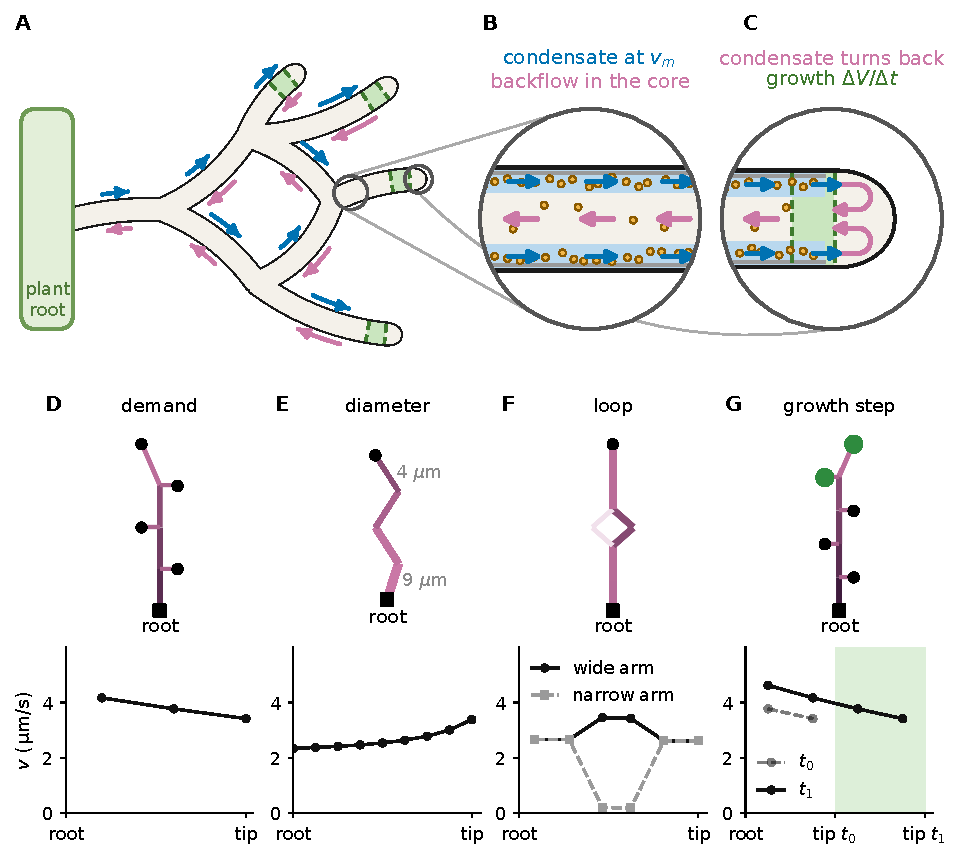
\includegraphics[width=\textwidth]{figures/Figure_4_v6.pdf}
 \caption{\textbf{Our model, showing motor flows moving toward the tip, and turning back as pressure-based flows. Model qualities are shown in the second row.}
\textbf{(A)} Schematic of the model: tipward flow (blue) returns as rootward flow (pink).
\textbf{(B)} The motor-driven condensate layer (light blue) along the hyphal wall, lipid droplets (yellow) in water, moves as a whole at speed $v_m$ (blue arrows), with a backflow of cytoplasm (pink) in the core, which can also carry some lipid. 
\textbf{(C)} At the tip, the condensate layer turns back, and the hypha grows at a rate $dV/dt$, calculated with a cylindrical volume.
\textbf{(D-G)} Various model qualities: (D) Demand accumulation along a uniform backbone with side tips; (E) Diameter tapering from 9 to 4 um along a single path, with fixed demand; (F) Loop between two junctions, with two arms of equal diameter, one twice as long as the other; (G) Growth step, with two more tips grown. Top row: network schematics; bottom row: rootward speed $v$ ($\mu$m/s) from the root to the tip; in (G) the network at $t_1$, with the hyphae grown since $t_0$ in green, and the profile at $t_0$ and $t_1$ with the growth in between shaded.}\label{fig:schematic_model}
\end{figure}

\subsubsection*{Single-pipe model: a moving condensate layer drives a central backflow}
\paragraph*{A condensate layer at $v_m$ leaves an inner tube for water}
We imagine that a flux of condensate containing lipid driven by motors throughout the aseptate mycelium could trigger large movement of the cytoplasmic fluid in both the direction of the lipid due to viscous friction and the other direction due to the incompressibility of the fluid in the case where no water could flow out of the hyphae.
As such, the condensate, a water-oil-like emulsion of lipid droplets of higher viscosity, forms a layer that uniformly coats the internal surface of the hyphal pipe. We assume the speed profile of the condensate layer in its cross-section is uniform, which can be explained by the effective viscosity, and the drag of the condensate layer on the water in the core of the hyphae. The condensate layer has a volumetric proportion $\theta$ of lipids and $(1-\theta)$ of water, and moves at a speed $v_m$. In this model, we also imagine that the condensate layer is coating the walls, and that the water in the core of the hyphae is free to flow at a rate of $q_{w,r<a}$, with a radius $a$ smaller than the hyphal radius $b$. The volumetric proportion of lipids in the whole pipe is $\Theta$, which is related to $\theta$ by $\Theta = \theta (b^2 - a^2) / b^2$.

By solving the Navier-Stokes equation in the inner pipe, setting the boundary conditions to be $v_m$ at the border of the inner pipe, one can determine the radial speed profile $u(r)$ in cylindrical symmetry to be 

\begin{equation}
\label{eq:speed_profile_main}
u(r) = v_m + \frac{2(q_{w,r<a} - \pi a^2 v_m)(a^2 - r^2)}{\pi a^4}.
\end{equation}

The flow of water through the inner pipe can be written as

\begin{equation}
\label{eq:net_inner_flow}
q_{w,r<a} = q_w - \pi b^2 \Theta \frac{1-\theta}{\theta} v_m,
\end{equation}

where $q_w$ is the net flow of water through the whole pipe.
Interestingly, when one assumes $q_w = 0$ as would be the case in a closed pipe system, we have:
\begin{equation}
\label{eq:max_speed}
u(0) = -v_m\left(1+2\frac{\Theta(1-\theta)}{\theta-\Theta}\right) .
\end{equation}

This result suggests a possible explanation for the bidirectional movement that we observe.
For all values of $\Theta$ and $\theta$, we have $u(0)$ which is of opposite sign compared to $v_m$.
It also suggests a possible explanation for the spatial and temporal variation of speeds.
The spatial variation of $\Theta$ (SI Fig.~\ref{fig:theta_spatial}) indeed directly contributes to the magnitude of the backflow speed.
Where a larger share of the lipid moves to the tip, the return flow is faster (Spearman $\rho = 0.40$ within plates, also after accounting for tip distance), as the model predicts (Eq.~\ref{eq:max_speed}: the backflow rises with $\Theta$).

\subsubsection*{Network model: pipes as circuit elements}
\paragraph*{Each pipe is a flux source in parallel with a resistor}
Our conceptual model seemed to be supported by the data at the individual pipe level.
Cutting a segment out of the network brings the nearest tip closer, which in the model lowers the motor speed and with it the backflow, as observed after section cuts, where both streams slowed by about a fifth (Fig.~\ref{fig:perturbations}C).
However, we wanted to know what its consequences would be at the network level.
Could it explain the observed variation of speed in space and time?
When establishing the speed profile through the pipe, we were also able to derive the pressure gradient along the idealized hyphal pipe.
Because fluid movement happens at low Reynolds numbers in our system and the entrance length in each individual hyphal pipe is close to its diameter, the approximation of an infinite length cylinder we used to derive flow profile in a single pipe is still justified in the network context.
A network of connected pipes is then analogous to a network of these individual circuit elements.

Such an electrical circuit equivalent of the network can be solved with linear algebra using Kirchhoff's law at each intersection, and requiring that the sum of pressure drops around loops in the network be zero (Methods). 
As in the case of growth induced mass flow discussed above in \nameref{subsec:si_mass_flow}, we set the sink magnitude at each node to correspond to newly created volume $\Delta V_k$ and added a global reservoir, connected to manually annotated nodes which are strongly suspected to be connected to roots.  This volume can be though of as the minimal volume which needs to be transported to the tips to have sustained growth. Using lipid dry mass measurements, we can estimate the volume amount of lipid $J_l$ that needs to be transported to the tips to sustain growth (Methods, \nameref{subsec:si_lipid_fraction}). This allows us to set the sink magnitude at each node in the network. Additionally, we assume that the network is interested in the energy minimization of the flow, which is equivalent to minimizing the total power dissipation in the network. This allows us to solve for the pressure at each node in the network, and therefore the demand $J_l$ through each edge.

In each edge the lipid current fixes the size of the motor-driven condensate: with a lipid share $\theta$ of the condensate (set to 0.05) moving at the motor speed $v_m$, $J_l = \pi(b^2 - a^2)\theta v_m$, so the core radius follows from $a^2 = b^2 - J_l/(\pi v_m \theta)$, so an edge that carries more lipid has a thicker condensate and a narrower core. The sign of $J_l$ determines the direction of motor flow. The condensate and the core it drags along carry a volume 

\begin{equation}
q_s = \pi v_m\left[(1-\theta)(b^2-a^2) + a^2\right]
\end{equation}

towards the tips. Each edge then acts as a source of flux $q_s$ in parallel with the hydraulic conductance of its core, $K = \pi a^4/(8\mu L)$, so that its net water flux is $q_w = q_s - K\Delta p$ (Methods), where $\Delta p = p_j - p_i$ is the pressure difference along the edge from node $i$ to node $j$, the direction in which $q_s$ and $q_w$ are counted. These values are all derived from the previously solved $J_l$, and we use them in a second solver to find the backflow. Solving these elements together for the pressures, with no water entering or leaving the network except at the roots, which are tied to a common reservoir (growth is neglected here, as it moves far less volume than the motors), gives $q_w$ on every edge, and with it the pressure-driven return through the core, $q_c = q_s - q_w$. We compare the mean speed of this return, $|q_c|/(\pi a^2)$, with the measured rootward speed. Centerline speed $u(0)$ would be the speed at the center of the pipe, which we do not expect to measure reliably. The model uses only measured or physical inputs: the network and its growth from the time-lapse, hyphal widths from the network images recalibrated on the filmed hyphae, the measured tipward speed, and $\theta = 0.05$ with $a \geq 0.8\,b$; nothing is fitted to the rootward speeds.

% NOTE (16 Oct, shortened 17 Oct): 'nothing is fitted to the rootward speeds' here contradicts the Fig 5 paragraph and caption, which now say theta was chosen by a sweep scored on the rootward speeds (75.4-77.6 % within 2x for theta 0.02-0.3).
In the model, $v_m$ is given by a calibrated function of the network distance $d$ to the nearest growing tip, $\hat{v}_m(d) = v_\infty - (v_\infty - v_{\mathrm{tip}})\,e^{-d/\ell}$, fitted to the measured tipward speeds, with $v_\infty = 3.10~\mu$m/s, $v_{\mathrm{tip}} = 2.14~\mu$m/s and $\ell = 1.71$~mm (Fig.~\ref{fig:fig5_plug}b; Methods). The model predicts the rootward speed on 1,544 bright-field edges in 15 sessions with a median fold error of 1.45. 

A number of properties can be shown in toy networks (Fig.~\ref{fig:schematic_model} D-G).
Tree networks aggregate backflow into their central trunk, increasing flow rate (Fig.~\ref{fig:schematic_model}D).
This increase in flow rate can increase backflow speeds, if not modulated by a greater flow capacity, which can be done by increasing the inner diameter (Fig.~\ref{fig:schematic_model}E). These two properties in tree-like networks are the basis for the observed increase in rootward speed with distance from the tip (Fig.~\ref{fig:asymmetries}B).
One feature this model also predicts is circularity in added loops, specifically if these have a resistance imbalance. A length or diameter difference between two arms of a loop can create a circular flow, with a faster arm returning to the trunk and a slower arm carrying a net flow to the tip (Fig.~\ref{fig:schematic_model}F). This also concentrates the backflow in the wider or shorter arm.
Finally, as tips grow, they increase their demand for lipid, which increases the motor streaming and with it the backflow (Fig.~\ref{fig:schematic_model}G). These toy models were constructed with typical measured values of hyphal diameter, tipward speed, and tip distance, and show that the model can illustrate the mechanism in backflow speed variation across the network.

\begin{figure}
    \centering
    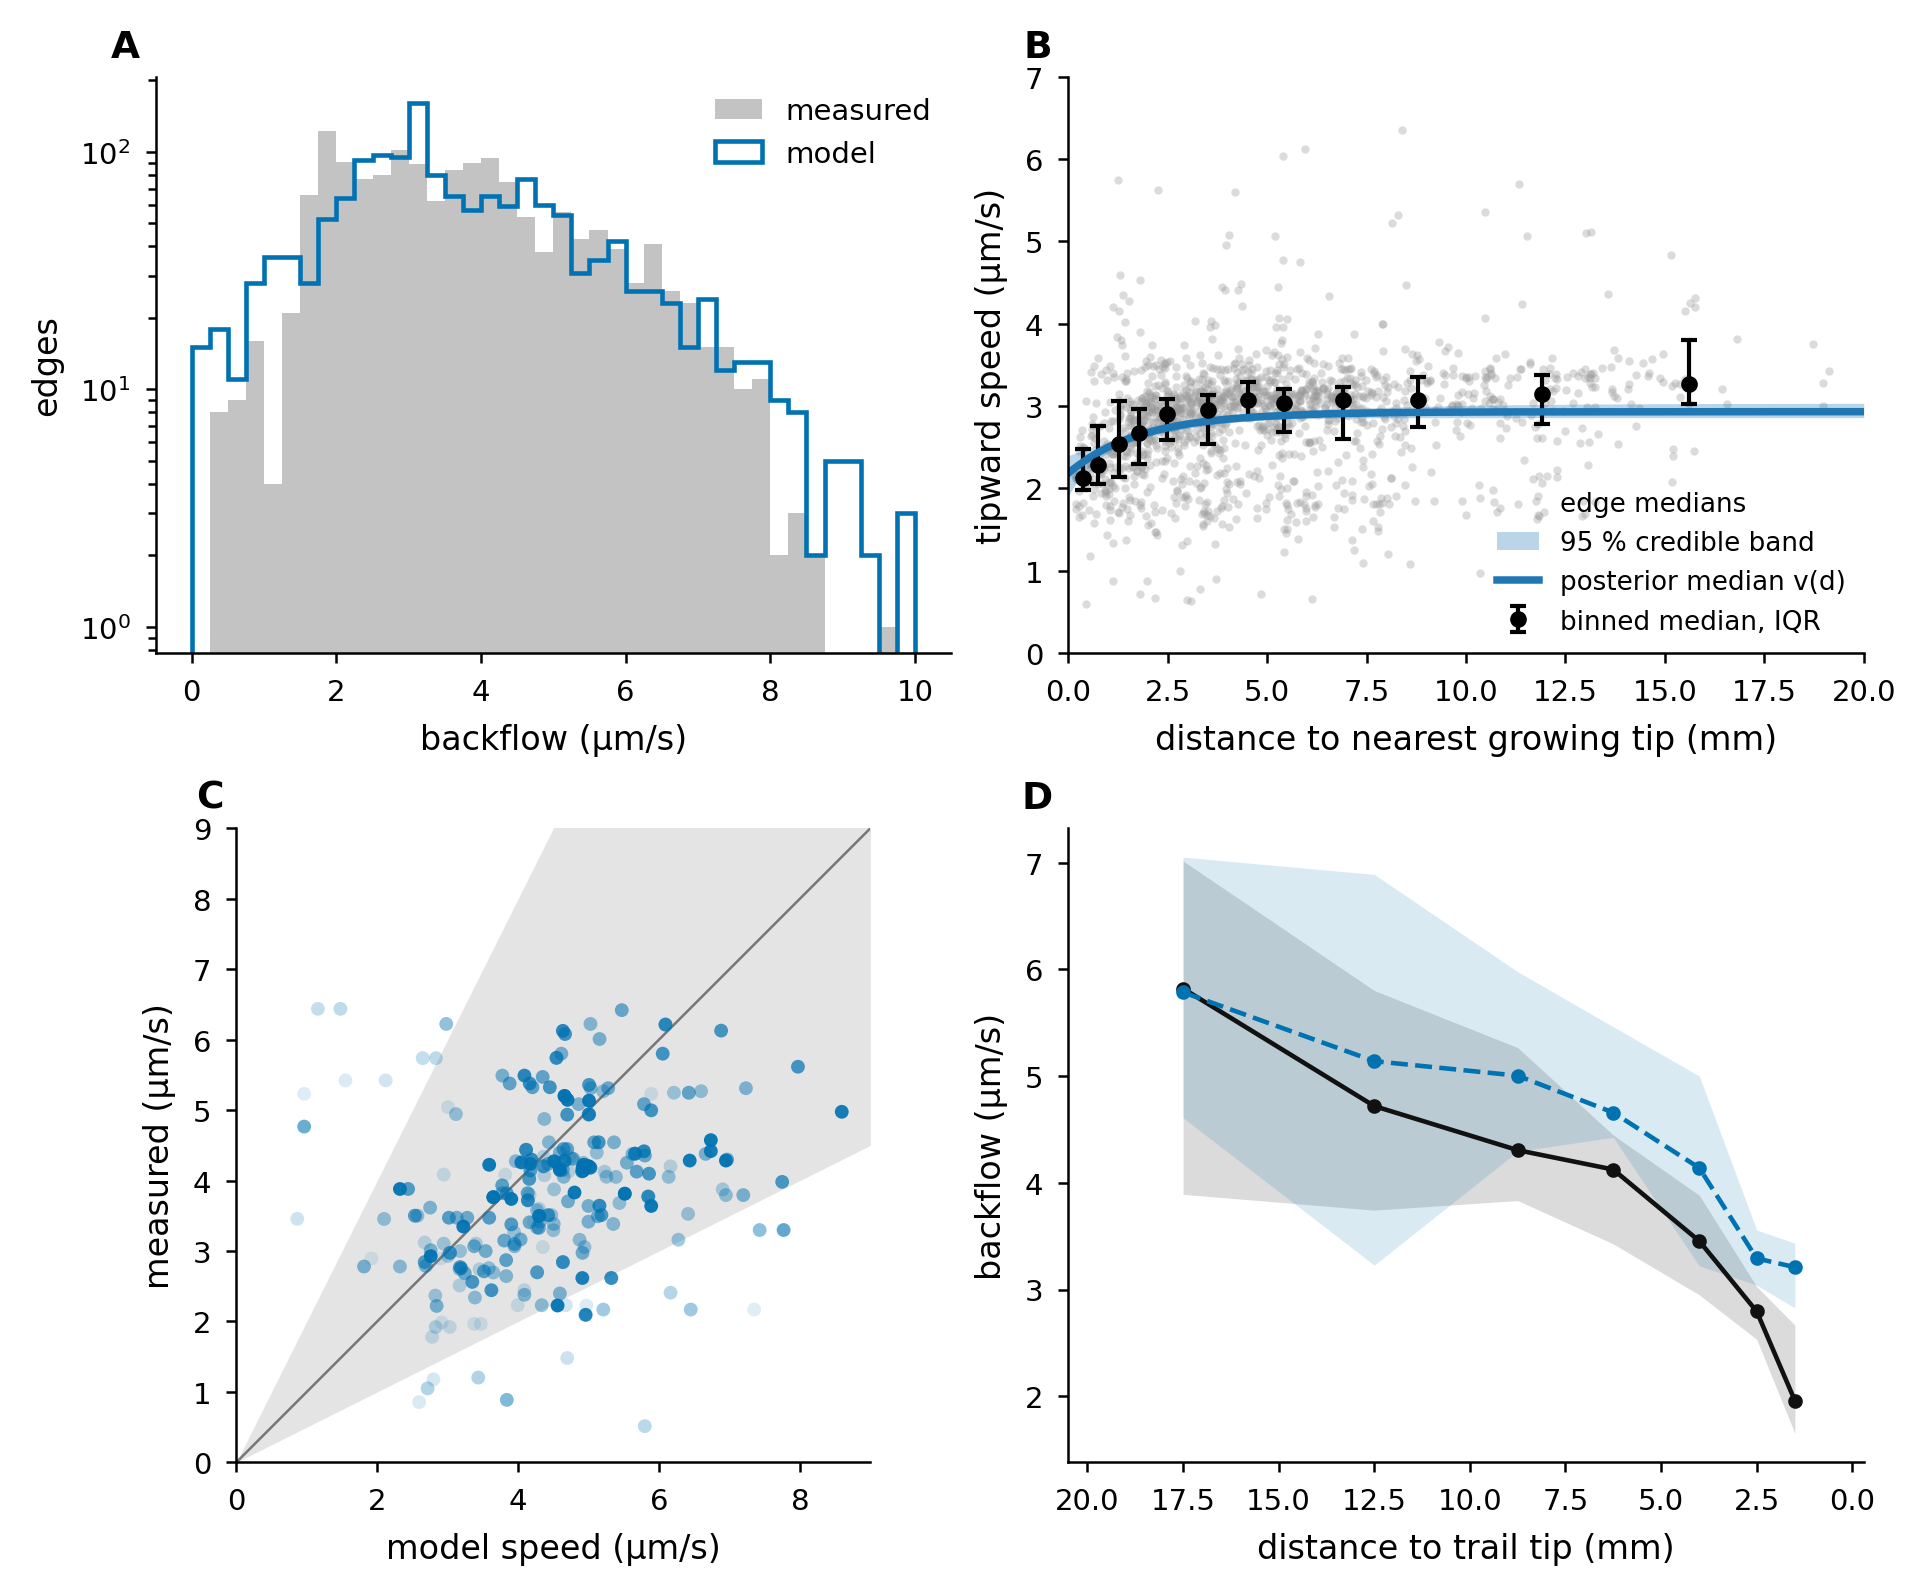
\includegraphics[width=\linewidth]{figures/fig_plug_model.png}
    \caption{\textbf{The network model reproduces the distribution of rootward speeds and their rise away from the growing tips.}
Measured bright-field speeds (grey, black) against the model (blue): global pressure solve with motors at the tipward speed profile of (b), physical inputs only, apart from $\theta$, chosen by a sweep scored on the rootward speeds (Methods).
\textbf{(A)} Distribution of the rootward speed over every measured edge, measured (grey bars) and modelled (blue line), counts on a log axis (1,544 edges in 15 sessions on 5 plates); speeds of 10~$\mu$m/s and above fall in the last bin.
\textbf{(B)} Tipward speed against distance to the nearest growing tip: edge medians (grey, 1,481 edges), binned medians with 25th--75th percentile (black), and a hierarchical Bayesian fit of $v(d) = v_\infty - (v_\infty - v_{\mathrm{tip}})\, e^{-d/\ell}$ (posterior median and 95\% credible band, blue): $v_{\mathrm{tip}} = 2.18$ [1.92, 2.39]~$\mu$m/s, $v_\infty = 2.93$ [2.86, 3.03]~$\mu$m/s, $\ell = 1.85$ [1.11, 3.52]~mm (SI, \nameref{subsec:si_forward_flow}).
\textbf{(C)} Measured against modelled rootward speed on the 274 trail segments within 10~mm of the trail tip, each as the median over the trail's segments within $\pm$0.5~mm (measured: of the measured segments only): 88\% within a factor 2, median ratio of modelled to measured 1.17.
Paler points have a larger uncertainty (the measured interquartile range and the range of the model within $\pm$0.5~mm along the trail, combined); grey wedge: within a factor 2; line: identity.
\textbf{(D)} Rootward speed on trail segments against the distance to the trail's tip at the session, in bins of 0--1, 1--2, 2--3, 3--5, 5--7.5, 7.5--10, 10--15 and 15--20~mm holding 3, 14, 19, 65, 73, 100, 130 and 88 measured segments; line: bin median, band: 25th--75th percentile (grey: measured, blue: model).}\label{fig:fig5_plug}
\end{figure}

The model allows us to predict on each edge what the net volumetric rate of fluid movement $q_w$ would be and then the direction and magnitude of the flow speed in the inner tube of each edge of the network (Fig.~\ref{fig:fig5_plug}).
We found that our model captures salient features of the bidirectionality of flow observed across all edges. One important result is that we are able to capture the distribution of rootward speeds across the network (Fig.~\ref{fig:fig5_plug}A), with 77.5\% of the 1,544 measured rootward speeds within a factor of 2 of the modelled speeds, and a median ratio of modelled to measured speed of 1.06. This was achieved by fitting only one parameter ($\theta$; SI, \nameref{subsec:si_model_variants}) to the measured rootward speeds, and only using physical inputs and the measured tipward speeds. The model also captures the rise in rootward speed with distance from the nearest growing tip (Fig.~\ref{fig:fig5_plug}D), which is a key feature of the observed flows (Fig.~\ref{fig:asymmetries}B). An important element of this rise is also the tipward speed falloff, which was estimated with a hierarchical Bayesian model (Fig.~\ref{fig:fig5_plug}B; SI, \nameref{subsec:si_forward_flow}). Along the filmed trails, the model predicts which trails carry faster backflow (Spearman $\rho = 0.50$ between modelled and measured trail medians, 30 trails, $p = 0.005$; Fig.~\ref{fig:fig5_plug}C), and the rise in rootward speed away from the tip has the same sign in 11 of 14 trails, although the modelled rise is shallower than the measured one.

A number of other correlations also emerge from the model (SI, \nameref{subsec:si_tree_loop}; SI Fig.~\ref{fig:relations}). 
The network structure is a key determinant of the backflow speed, with the model predicting that edges with a higher betweenness centrality have a faster backflow speed. The model also predicts that edges with a larger share of lipid moving to the tip have a faster backflow speed, which is consistent with the observed correlation between lipid share and backflow speed (Spearman $\rho = 0.40$ within plates, also after accounting for tip distance). We also define a measure of edge network density or robustness $\kappa$ as the number of cuts needed to disconnect the network section within 0.25 to 1~mm of an edge from the root, averaged over these section sizes. While the model does not reproduce the observed correlation between $\kappa$ and backflow speed, this could be observational bias, as the measured trails are not a random sample of the network, but largely high edge-betweenness edges (SI, \nameref{subsec:si_video_selection}). Edges with high $\kappa$ but low edge betweenness are less likely to be filmed, and therefore less likely to be included in the analysis. The model does generally over-predict the backflow speed on high-betweenness edges, and therefore underestimates the speeds measured in edges with high $\kappa$ and low betweenness (SI Figs.~\ref{fig:tree_loop},~\ref{fig:kappa}).

Some other shortcomings are that the model assumes a uniform flow within hyphae, and does not account for the existence of observed sparse flows (SI, \nameref{subsec:si_flow_regimes}). These are edges where only sparse particles are seen moving in either direction. The model assumes full flow in all hyphae, and cannot describe these phenomena. 

Hyphal diameter is also a key determinant of the backflow speed, with the model predicting that edges with a larger diameter experience more demand, and therefore have a faster backflow speed. This is consistent with the observed correlation between hyphal diameter and backflow speed (Spearman $\rho = 0.53$ within plates, also after accounting for tip distance) (SI, \nameref{subsec:si_widths}; SI Fig.~\ref{fig:relations}). This result was obtained by using the measured hyphal diameters in the videos, which is more accurate than the network diameters, obtained on 2x microscopes.
% NOTE (17 Oct): Check the magnification of the network imaging ('2x'). 

\subsubsection*{The lipids form an emulsion separate from the bulk cytoplasm}
Even our estimate of 5\% of the cytoplasm filled with lipids suggests that a significant proportion of the volume of the hyphal is filled with lipids.
Such a proportion could easily lead to clogging if all of the lipids coalesce into a single phase.
What then is this large fraction of neutral lipid packaged within the cytoplasm?
The minimal unit of lipid packaging is generally thought to be membrane bound lipid droplets.
Such lipid droplets are generally kept from coalescing by coating~\cite{thiam_why_2017}.
The ensemble of those lipid droplets can then form an emulsion with a set lipid volume fraction.
The emulsion phase, due to the repulsive strength between the different lipid droplets, can have different rheological properties than the rest of the cytoplasm~\cite{jeffrey_rheological_1976}.
We assume that this emulsion is phase-separated from the bulk cytoplasm.

\namedsubsection{Lipid generated backflow}{subsec:res_backflow}

\begin{figure}
    \centering
    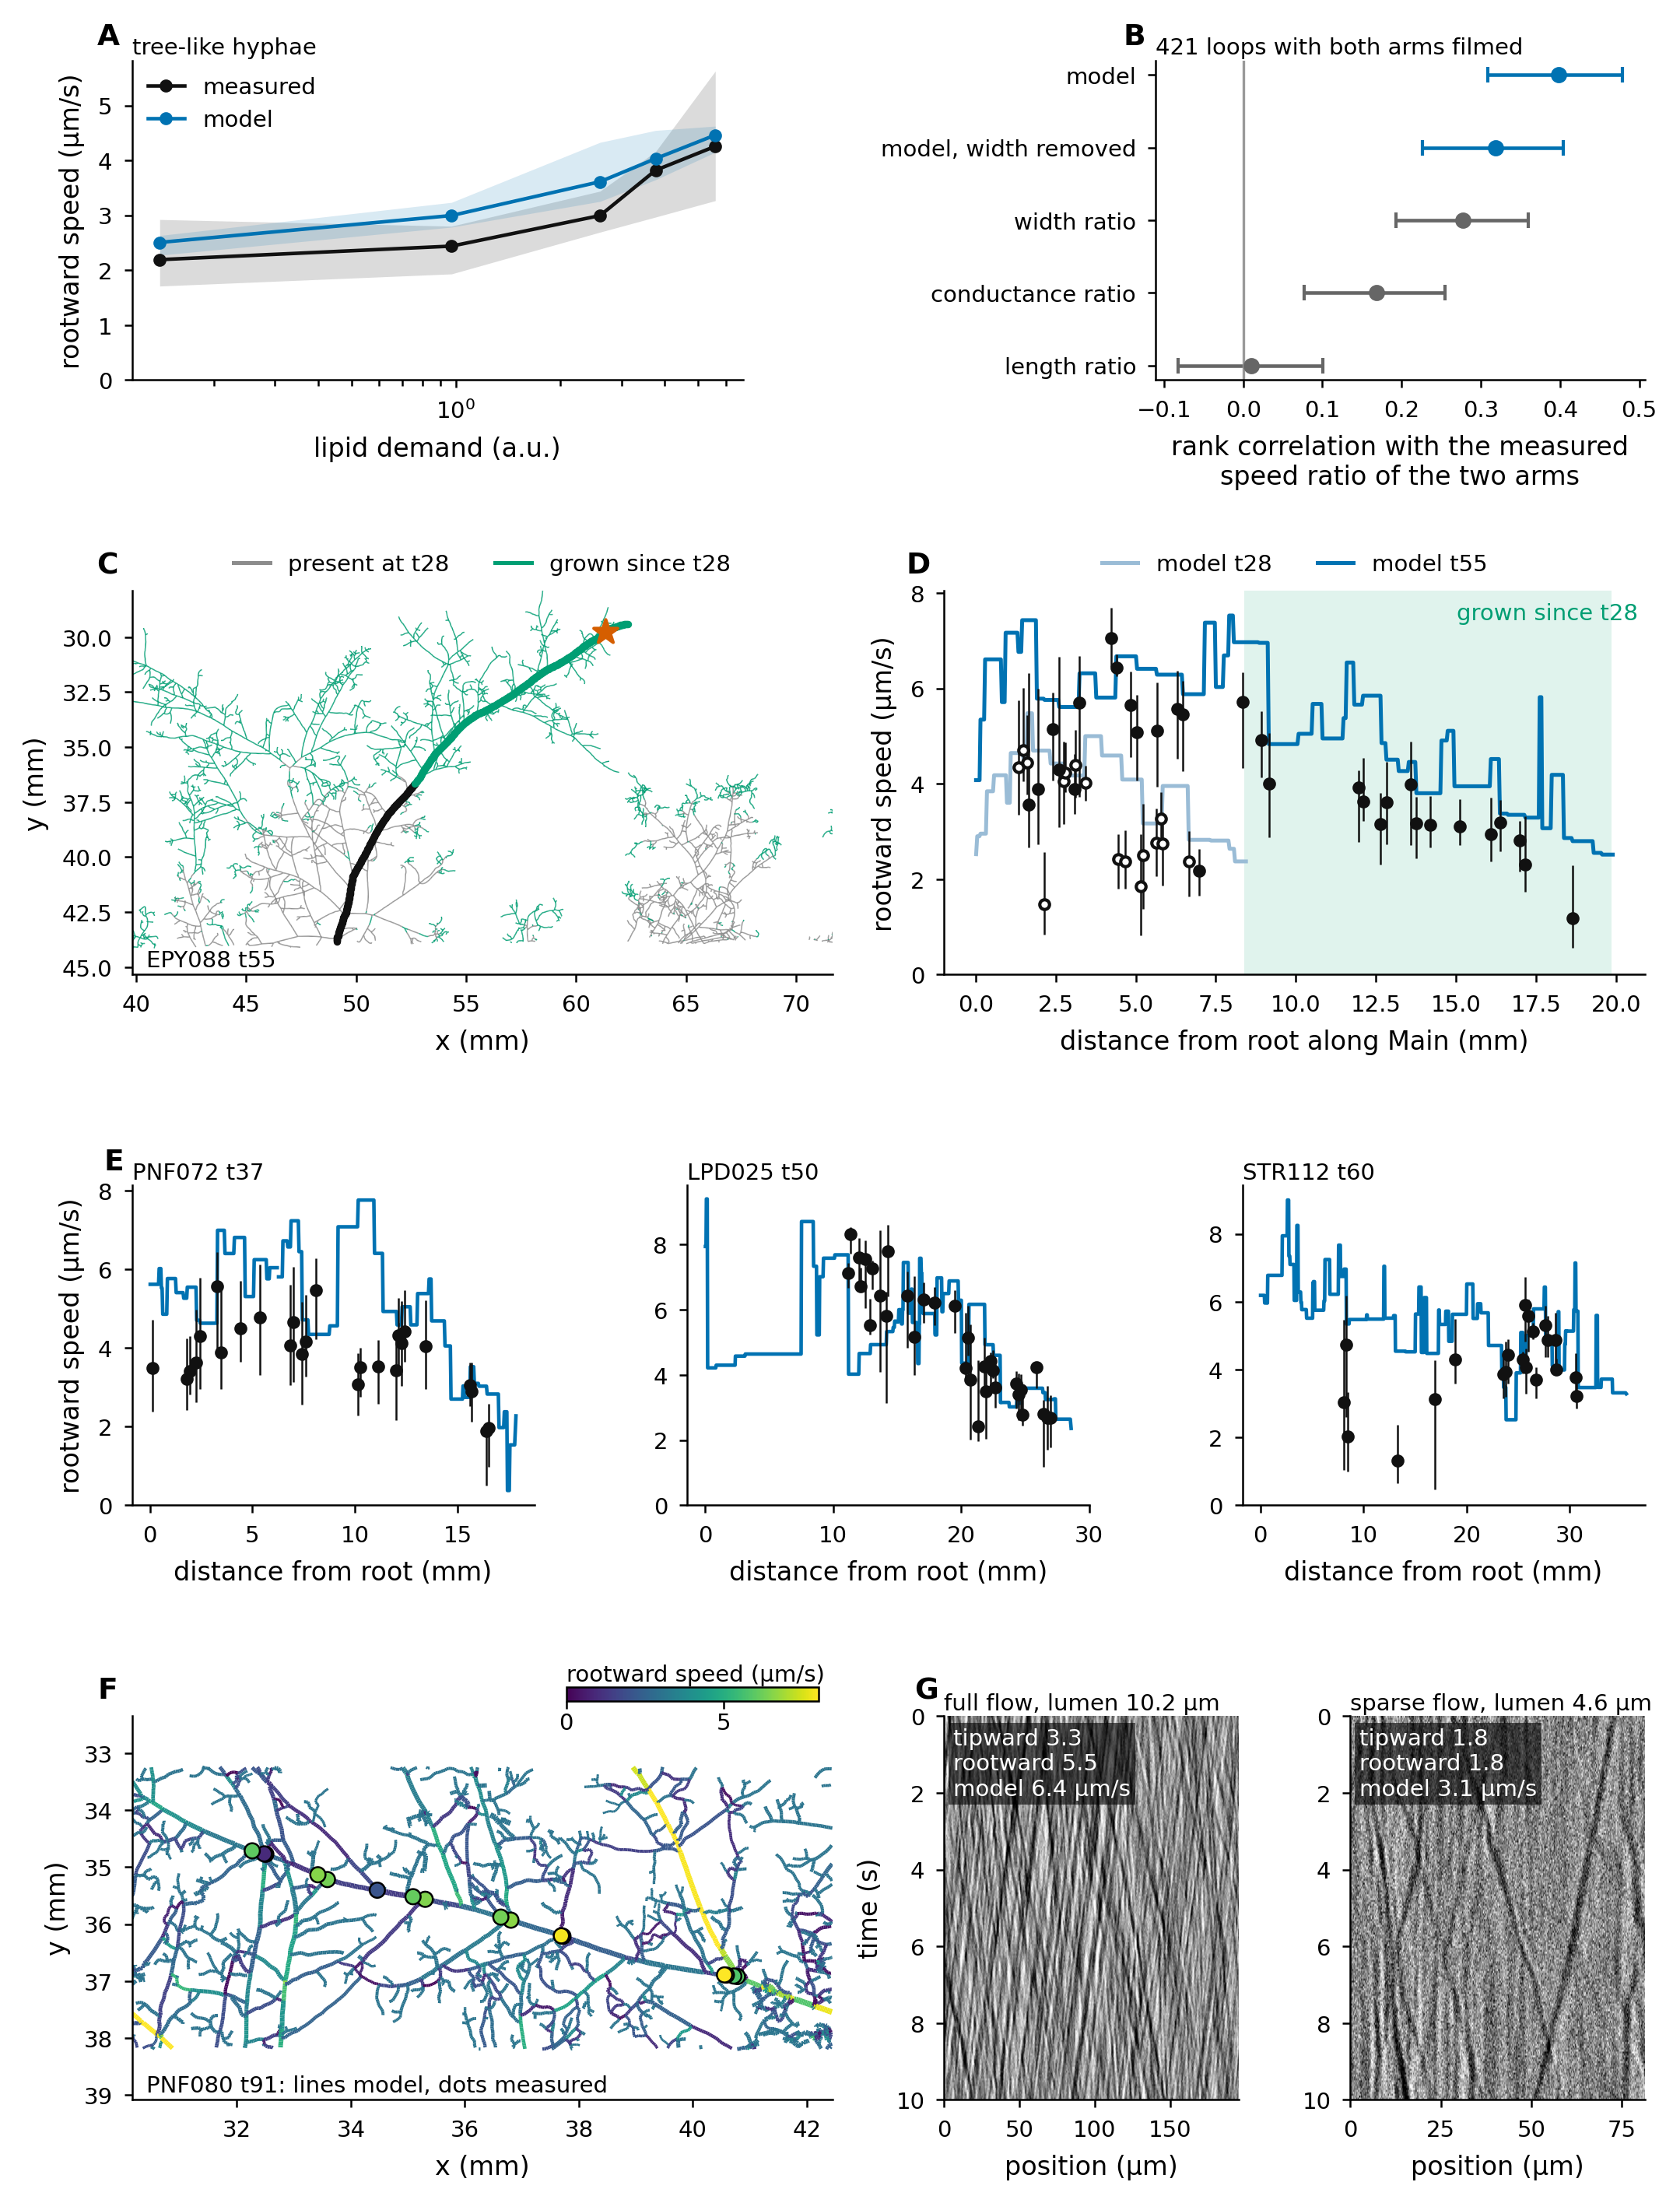
\includegraphics[width=\linewidth,height=0.64\textheight,keepaspectratio]{figures/fig6_model_examples.png}
    \caption{\textbf{Network-level tests of the model's predictions (Fig.~\ref{fig:schematic_model}D-G).}
Model as in Fig.~\ref{fig:fig5_plug} (blue); measured bright-field rootward speed per trail segment, median with 25th--75th percentile (black).
\textbf{(A)} Tree-like hyphae: rootward speed against the routed lipid demand, medians of the five demand quintiles with 25th--75th percentile, measured (black) and model (blue); the model is within a factor 2 of the measurement on 94\% of these edges.
\textbf{(B)} Loops with both arms filmed (n=421): rank correlation with the measured rootward speed ratio of the two arms, for the model, for the model with the arms' width ratio removed from both ratios (partial correlation), and for the width, conductance and length ratios of the two arms, with bootstrap 95\% intervals.
\textbf{(C)} Network of EPY088 at session t55, every hypha coloured by whether it was present at t28 (grey) or grew since (green), with measured trail in bold and its tip (star).
\textbf{(D)} Rootward speed along measured trail against the distance from the root, model at t28 (light blue) and t55 (blue; running median over 5 segments), measured at t28 (open) and t55 (filled); green: grown since t28.
\textbf{(E)} One trail on each of the other plates: PNF072 t37 Middle (26 segments, 92\% within a factor 2), LPD025 t50 Middle (32, 94\%) and STR112 t60 LeftMiddle (21, 86\%).
\textbf{(F)} Where the model sends a hypha's return elsewhere: trail LeftMiddle of PNF080 at t91, 8 to 19~mm from the root, every edge coloured by the modelled rootward speed (line width proportional to hyphal width) and the 16 measured segments by the measured one, on the same scale.
Measured: median 6.3~$\mu$m/s to the root and 3.3~$\mu$m/s to the tip; model: 2.1~$\mu$m/s, because the pressure solve returns only 0.66 (interquartile range 0.47--0.79) of the trail's motor stream through its own core and sends the rest back through neighbouring hyphae.
\textbf{(G)} Full and sparse flow: bright-field kymographs of two edges of PNF080 at t81, both more than 6~mm from a growing tip (moving signal only, time mean removed; 20 frames per second).
Left, full flow (lumen 10.2~$\mu$m): tipward 3.3, rootward 5.5, model 6.4~$\mu$m/s; right, sparse flow (lumen 4.6~$\mu$m): few, faint streaks at 1.8~$\mu$m/s in both directions, model 3.1~$\mu$m/s (SI, \nameref{subsec:si_flow_regimes}).}\label{fig:fig6_examples}
\end{figure}

\subsubsection*{The model reproduces characteristic features of the measured flows}
    
% NOTE (17 Oct, facts behind this subsection not in the prose): (A) 94 % of the 111 tree edges are within a factor of 2 (rank correlation 0.65); at fixed demand no width effect is detectable on tree edges (measured +0.21 [-0.42, 0.84], model -0.05), but over all filmed edges the video lumen keeps a width effect at fixed demand (within-plate rho 0.43 measured, 0.16 model). (B) The model exaggerates the arm difference (SD of the log ratio 0.89 against 0.53); SI figures for the loop density plot and the side branches are built, not yet placed. (C-D) 70 % of the t55 network length grew after t28. (F) With the betweenness/kappa split at the medians, the model is low on high-kappa, low-betweenness edges (log2 model/measured -0.35; 2.97 against 3.80 um/s, 364 edges) and high on low-kappa, high-betweenness edges (+0.31; 4.47 against 3.53, 427 edges). (G) Sparse-flow edges: median lumen 6.2 against 8.4 um for full flow.

We compare the model's characteristics, listed in Fig.~\ref{fig:schematic_model}D-G, with the measured flows in the network (Fig.~\ref{fig:fig6_examples}A-G). The first is the claim that in tree-like parts of the network, lipid demand accumulates towards the root, and that this accumulation increases the backflow speed. We find that in the 111 tree-like edges (on no loop) that carry routed lipid demand, the measured rootward speed rises with the demand as the model predicts: effect of log demand on log speed 0.11 [0.05, 0.18] measured against 0.13 [0.10, 0.15] in the model (Fig.~\ref{fig:fig6_examples}A).  


The second is the claim that in loops, the model predicts which arm carries the faster backflow. We find that in 421 small loops with both arms filmed, the model predicts which arm carries the faster backflow (Spearman $\rho = 0.40$ [0.31, 0.48] between modelled and measured arm speed ratios), also beyond the arms' width ratio (partial $\rho = 0.32$) and when the filmed arms are more than 150~$\mu$m apart ($\rho = 0.44$, 158 loops). The width ratio alone gives $\rho = 0.28$, the conductance ratio $\rho = 0.17$ and the length ratio $\rho = 0.01$: the routing of the network solve, not arm length, sets which arm is faster (Fig.~\ref{fig:fig6_examples}B).


The third is the temporal change in backflow speed along a trail as the network grows. On EPY088 Main, the stretch that existed at t28 speeds up from t28 to t55 by 1.51-fold in the model and 1.71-fold measured (medians 4.17 to 6.29 and 3.01 to 5.14~$\mu$m/s; 16 and 15 segments); at t55, 90\% of the 30 measured segments are within a factor of 2 of the model (Fig.~\ref{fig:fig6_examples}C-D). The mechanism is the one of Fig.~\ref{fig:schematic_model}G: demand rose 3.3-fold, the extra lipid thickens the condensate layer, and the return rises although the hypha also widened.


We also show other examples of the model's predictions on other plates (Fig.~\ref{fig:fig6_examples}E). One trail on each of the other plates: PNF072 t37 Middle (26 segments, 92\% within a factor of 2), LPD025 t50 Middle (32, 94\%), STR112 t60 LeftMiddle (21, 86\%). Over the 30 trails with $\geq$5 segments, the model ranks the trails by their median rootward speed ($\rho = 0.50$, $p = 0.005$), but orders segments within a trail only weakly (median within-trail $\rho = 0.15$).

% NOTE (16 Oct, summarized 17 Oct, Fig 4F, other tests): Side branches along the trunks (62 filmed junctions, junction_side_branches.py): the model ranks the side / through speed ratio (rho +0.35, +0.30 beyond width), but its sign (46/62) does not beat the rule 'the side branch is slower' (49/62). Null: the trail's share of local conductance over 1 mm (rho -0.07 after tip distance and demand); 19 junctions with two rootward legs (9-10 of 19 right).

One reason the model sometimes shows different backflow speeds than measured is that the global pressure solve can send part of a hypha's return elsewhere. On PNF080 t91 LeftMiddle (8--19~mm from the root) the model returns only 0.66 (IQR 0.47--0.79) of the trail's motor stream through its own core and circulates the rest through side hyphae, giving 2.1 against 6.3~$\mu$m/s measured (Fig.~\ref{fig:fig6_examples}F). This is the other face of the betweenness/$\kappa$ result above: the model concentrates the return on main routes and misses the faster flow through well-connected sections.

Finally, one state of flows that is not representable by the model is sparse flow (13\% of edges, thin, $\sim$1.8~$\mu$m/s both ways); the model over-predicts these edges (bias 1.60; SI, \nameref{subsec:si_flow_regimes}; Fig.~\ref{fig:fig6_examples}G). In the kymographs, these sparse flows largely show long straight trajectories of single particles, not part of a condensate. This violates the model's assumption of particles moving together in tight flows. 

% NOTE (16 Oct, summarized 17 Oct, Fig 4F and circulation): In the 2x toy loop a third of the motor flux circulates (up the long arm, down the short one), while the long arm's core still flows rootward; the core reverses only from ~4x. In the real networks (main model) the core flows tipward on 0.5-2.6 % of edge length, although loop arms carry a median net flux of 30 % of their motor flux. The real geometry reduces circulation relative to width or length shuffles on all five plates (loop_geometry_null.py). No data in the paper show loop circulation itself; the circulation point is for the Discussion (note there).
% NOTE (15 Oct, summarized 17 Oct, Fig 6D): On the t28 stretch of EPY088 Main, demand rose 3.3-fold, the lumen area b^2 1.36-fold and the core area a^2 1.06-fold, so the extra cross-section went mostly to the condensate layer and the return rose 1.56-fold. Caveat: our data do not show widening following demand (lagged demand-width correlation ~0 at every lag; demand_rise.py, demand_widening.py). LPD025 Middle is the only other trail with enough segments in several sessions (7-10 each).
% NOTE (15 Oct, summarized 17 Oct, Fig 6F; fig_outputs/flow_regime/pnf080_investigation): In the model the trail's net flux points tipward on 9-18 mm, a ~10 mm circulation loop (volume enters at ~8.8 mm through a side branch and leaves into side hyphae at 17-21 mm); measured, the return there (6.5 um/s) exceeds even a full return of the motor stream (~3.5 um/s). Not explained by nearby growth; past demand raises the model to 2.9 um/s, splitting crossings to 2.2, idle motors change nothing.

\subsubsection*{One physical model from pipe to network, with consequences for trade}
Our simple physical model can therefore explain a wide variety of our experimental observations.
At the single hypha level, it provides an explanation for bidirectional fluid flow.
At the growing network level, it is compatible with the observed non-trivial spatio-temporal variations in flow speeds.
Such a physical explanation of bidirectional transport in AM fungal networks has direct consequences on symbiotic trade.
Because the movement of lipids generates fluid flow in the reverse direction, the proportionality of resource exchange could emerge directly from this physical coupling. 
% NOTE (15 Oct, main-text review): See the C/P notes in the Discussion: the returning volume is proportional to motor-carried carbon by construction, not to growth carbon.

 % We wanted to know whether the lipid movement induced backflow could explain the proportionality of resource exchange. We assumed that the concentration of phosphorus in the water of the inner tube was constant and that the input carbon flux varied. We found that, under this assumption, the carbon flux from the plant and the phosphorous flux from the fungal colony were maintained proportionally (Fig. \ref{fig:hydraulic_proportionality}b). To obtain a proportionality factor of $1/3$ $\mu g$P / $\mu g$C, as previously found (see Chapter \ref{chapt2}), we had to set the concentration of P to $\approx 1.9 mol/L$ which is much higher than the concentration typical found in plant cells of 5-20$mmol/L$ \cite{bieleski_phosphate_1973}.

\section*{Discussion}
% NOTE (11 Oct, structure): The Discussion lacks the C/P point the Intro sets up (L49; notes at the C/P paragraph below). The fluorescence detection-limit paragraph (pixel speeds 8-9 um/s) reads as Methods or SI material. Most of the rest is speculation (track orientation, supply-driven growth, aquaporins), which could be tightened around what the model leaves out.
% NOTE (12 Oct, for the Discussion; SI subsec:si_lipid_fraction): At v0 = 3 um/s the lipid flux needed for the observed growth fills a growing share of the hypha away from the tip (old analysis: up to ~4 % over ~10 mm; current measurement of the moving lipid share: 2.4 % within 2 mm of a tip and 4.6 % beyond 4 mm, transport_paper#94). Bago et al. measured ~24 % near the root and 0.5 % at the front (bago_translocation_2002, Fig. 3; the moved text cites the review bago_carbon_2000 with ~20 %). The point it supports is that transport at motor speeds lets the colony grow without filling hyphae with lipid, while at diffusive speeds (~0.1 um/s, commented-out estimate in the SI section) the needed fraction exceeds 100 %. This fits the supply-driven growth paragraphs.
\subsubsection*{Motor tracks form an oriented network}
\paragraph*{Lipids follow growth on polar filaments, an oriented graph}
Our results suggest that the lipids preferentially move in a direction informed by fungal growth.
% NOTE (15 Oct, main-text review): The main model now takes the motor direction from the GIMF solve, not the growth graph; the growth-graph direction matches the observed motor direction only slightly better on loops (86 against 81 %, 677 edges). Decide which story this section tells.
They also strongly support the idea that this movement of lipids could be actively driven by molecular motors moving in one direction on polar cytoskeletal filaments.
This network of filaments inside the fungal network is mathematically equivalent to a weighted oriented graph, where the weight of a given edge can represent the number of cytoskeletal filaments, allowing molecular motor movement.
It is unclear how this oriented network organizes to maintain a coherent intensity and polarity with growth. 
% NOTE (8 Oct, context in other organisms; guest_multiple_2026 now in PhD.bib, Curr Biol 36, full text read): The paper studies Filoreta ramosa, a reticulate (branching and anastomosing) amoeba. Actin protrusions explore, and microtubule uptake stabilises branches. Nuclei, lysosomes and mitochondria move both ways at 5.3, 7.3 and 8.3 um/s on microtubules; speed rises loosely with branch diameter (R2 0.54, 1.5-6.5 um; wider branches hold more MTs) and slows at nodes. Nocodazole lowers the maximum nuclear speed by 27 % and the run length by 33 %. The dynein inhibitor ciliobrevin D lowers speed by 70 %, and the remaining nuclei are still bidirectional. With latrunculin the change is < 25 %. MT nucleation (gamma-tubulin, GCP3) sits at branch nodes, not at nuclei. They contrast Physarum (pressure-driven streaming) with Filoreta (motors) as two network solutions; AMF here would use both, one per direction. Caveats: this is an amoeba with no wall or turgor, and it moves single organelles, not a lipid stream. Tipward speed against diameter in our data was requested from the 'Fluorescence slow bias?' session (8 Oct).
% NOTE (8 Oct): Our data show the same trend as Filoreta: the tipward speed scales as ~ D^0.5 (see the note at the summary paragraph). The rootward speed rises faster in bright-field (slope 1.09 [0.97, 1.20]; rootward/tipward ratio slope 0.62), but not clearly in Nile Red (ratio slope 0.16 [-0.05, 0.37]). The model uses a tip falloff of the motor speed, not v0(D); the diameter dependence is in SI subsec:si_forward_flow.

\paragraph*{Tracks likely inherit the orientation of tip growth}
Each edge of the network has a growth inherited orientation that is associated with the polarity of tip extension.
It is likely that part of the network of transport filaments simply orients in the direction of tip growth at the moment of its creation and persists in that direction over longer timescales.

\paragraph*{Rheological implications}
% NOTE (17 Oct): Speculative; the Discussion may be the better place for the yield-stress idea.
This points to the idea that the cytoplasm could be a yield stress fluid, which would have a different rheology than the condensate layer. 

\subsubsection*{Growth may follow supply}
\paragraph*{The system may be supply driven}
One way of thinking about the system is that it is mainly driven by supply.
Although in this paper our approach was to estimate what the flux of carbon was in each edge of the network from growth observation, it is possible that from the fungal point of view things work the other way around.
Growth would mainly emerge from the network's underlying molecular motor track organization.

\paragraph*{Supply-driven growth avoids an information bottleneck}
This has the advantage of solving an informational bottleneck.
If a tip grows at one end of the network, how is the information about its carbon demand transmitted to the root-fungal interface where that carbon will eventually come from?
Instead of needing information transmission to match supply and demand and orient carbon fluxes accordingly, fungal tips could grow and branch according to the carbon supply of the existing network of molecular motor tracks.
Indeed, the net flux of lipid across the colony could be entirely determined by its orientation (track direction) and intensity (number of parallel tracks assuming tracks are saturated with motors) as well as by the plant supply (source).
The growth might then simply occur at a rate limited by the network-determined supply of lipids.

\paragraph*{Topology changes need track reorganisation, which could send lipids both ways}
However, some abrupt topological changes, such as anastomosis or the colony abandoning growth in a specific region of space, could require a reorganization of the cytoskelal filaments.
It is unclear how that reorganization is modulated in a way that allows one to maintain a flux of carbon that is consistent with the general fungal growth strategy.
Depending on the timing of the reorganization, it is also likely that the flux of lipids moving on microtubules will not always follow the Kirchhoff law at some intersection.
Because lipids are incompressible and cannot accumulate in a node, this means that they will be recirculated in the internal cytoplasmic flow.
This phenomenon could explain the observation that lipids can also move in two directions in fungal hyphae.
% NOTE (8 Oct): Guest & Dawson 2026 (guest_multiple_2026) infer antiparallel MT arrays where branches growing from opposite directions fused (under nocodazole, such branches retract toward both nodes at once). This is another lineage in which anastomosis leaves tracks pointing both ways in one edge. In our model the motor direction comes from the hydraulic solve or from the growth direction (both open, Simon 8 Oct); there is no evidence of motor switching yet.

\subsubsection*{The detection limit explains only part of the slower rootward lipid stream}
Speeds taken from the orientation of all moving pixels, which do not depend on the streak detection and follow the true speed up to 8 to 9~$\mu m/s$ at 2 frames per second, still show a smaller rootward branch in fluorescence than in bright-field: the rootward stream is faster than the tipward stream by more than the 1.3-fold margin on 20\% of the fluorescence edges against 39\% of the same edges in bright-field (532 edges with both measured).
So the detection limit explains part of the lower fluorescence speeds in the rootward direction, but not all of them, and why the stained cargo returns more slowly than the bright-field backflow remains open (Methods, \nameref{subsec:fl_detection_limit}).
% NOTE (13 Oct, merged 16 Oct): This Discussion paragraph is a fluorescence against bright-field speed comparison (pixel speeds), so it falls under Simon's 13 Oct decision to drop such comparisons. It was moved here from the Results (Simon: 'this is for discussion'); on the 532 paired edges the numbers are 21 % against 39 %, and with both modes cut at 5 um/s 13 % against 17 % (the difference CI includes 0).

\subsubsection*{Mechanical coupling could make trade proportional; radius adaptation could control it}
% NOTE (15 Oct, Simon, for the Discussion): State that the global solve induces circulation around loops, which is not necessarily found in the data, but that a model like this is the best at redirecting flow into the central hyphae, raising their speed, which is what we measure. The supporting facts are that the global solve reproduces the upper half of the measured rootward distribution (95th percentile 7.15 against 6.82 um/s, KS 0.056), where locally coupled models (conveyor, junction cost) stay below ~4.7 um/s and give too little spread, and that the measured rootward speed rises away from the trail tips (Fig 5d) and correlates with betweenness (oyarte_galvez_travelling-wave_2025). Against it, its error grows with local loop density (Typst Fig 6D), and its too-slow misses are loop circulation. (16 Oct) Related: the network geometry works against circulation (Fig 4F note), and the measured backflow rises with network robustness kappa while the model does not follow; making every node near the image's bottom edge a root of the solve does not change this (SI subsec:si_tree_loop).
We see that bidirectional resource movement and trade could be largely mechanically mediated.
Such a control mechanism has the advantage of being robust because the proportionality of flow is embedded in the physical properties of the system and, therefore, does not require additional biological control.
However, in our model, the path taken by the phosphorus in the network is strongly dependent on its relative cumulative hydraulic resistance and, therefore, on the edge radii.
Radial adaptation could constitute a flow control mechanism.
However, we never observed hyphal external radii diminishing.
Full control would probably require an additional ingredient of radial shrinkage. 
% NOTE (9 Oct, C/P framing, Simon: frame on motor-carried carbon; transport_paper#128, analysis feat/cp-production fb436c6): In the global solve the volume returning into the roots equals the motor stream leaving them in all 15 sessions, so P out (constant [P]) is proportional to motor-carried carbon (theta times the motor stream) by construction (log-log slope 1.000). This is a property of the mechanism, not a fitted result. Against growth carbon it does not hold, with slope 0.19 (95 % CI -0.47 to 0.86, R2 0.03) over 15 sessions. On STR2307A112, growth carbon rises 4.7-fold over 5 sessions while the return stays flat (0.0050-0.0066 uL/h).
% NOTE (9 Oct, needed P concentration): With P:C = 1/3 to 1/4 ug P per ug C, motor-carried carbon at theta 0.05 needs [P] = 0.38 to 0.29 mol/L in the returning fluid, proportional to theta (0.19 mol/L at theta 0.025, 0.76 at 0.10). Plant cells have 5-20 mmol/L (bieleski_phosphate_1973; the range was not re-checked). Reaching 20 mmol/L needs theta ~0.0026, at which the motors carry ~0.19 times the carbon that growth uses (3.7 times at theta 0.05, median). So a plausible [P] and feeding growth pull theta in opposite directions. The old analysis (commented-out paragraph at the end of the Results) needed ~1.9 mol/L.
% NOTE (9 Oct, Bisot et al. 2026, full text checked, PMC12891005; bisot_carbon-phosphorous_2025): The exchange rate kappa = Phi_C / Phi_P is by MASS, ~3-4 ug C per ug P ('3 to 4 C/P'; Fig. 5 fronts at kappa0 = 3 and 4), and it is set by host genotype, not by fungal strain or P availability. Their carbon is EXPENDED carbon (CUE 50 %, i.e. twice the carbon built into biomass, spores included), a growth-based quantity, not the motor-carried carbon of this framing. Also, >= 85 % of absorbed P reaches the root within ~100 h (absorbed P would be ~30 % of fungal dry mass if none were transferred, against <= 4-5 % P measured in hyphae).

\subsubsection*{Aquaporins and osmotic pumping would extend the model, not contradict it}
In our model, we assumed that water could not flow out of the hyphae except at the hyphal-root interface.
However, it is likely that the ERM hyphae are covered with aquaporins that let water in and out.
% NOTE (5 Oct, Overleaf comments, L201): Simon: 'Maybe even not': AMF lacks genes associated with passive water-exchange hydroporins.
% NOTE (7 Oct, aquaporins): R. irregularis (then G. intraradices) has two functional aquaporins, GintAQPF1 and GintAQPF2 (Li et al. 2013, New Phytol 197:617-630, doi:10.1111/nph.12011): expressed in yeast, they speed the volume response to osmotic shock. This was found by web search, and the full text was not read; it was not in PhD.bib. It is now in PhD.bib as li_first_2013 (not yet cited).
In that case any kind of water potential gradient between the inside and outside of the hyphae could produce influx or outflux of water at any point of the network.
The resulting system would be analogous to the xylem-phloem system of plants.
In that case, the sugar loaded phloem generates an influx of water from the xylem.
This in turn generates a net flux of water through the phloem.
Any kind of osmolyte that would be produced inside the fungal network could very well drive a similar osmotic pump by changing the overall flow distribution in the network.
Although we cannot exclude such effects from playing a role in the transport of resources within the AM colony, it is not incompatible with the mechanism of bidirectional flow described in this paper.
Regardless of the contribution of other mechanisms, our results strongly suggest that lipid movement results in some fluid flow in the opposite direction.
And such backflows must be playing a significant role in the full picture of AM fungal flows.
The framework developed here can also be flexibly expanded to include the effect of other kinds of carbon demand, such as spore growth or hyphal maintenance.
By adding current generators at different places in the network to represent the influx or outflow of water due to water potential mediated flow of water through aquaporin, it is also possible to account for additional transport mechanisms.

\section*{Bibliography}
\bibliographystyle{bxv_abbrvnat}
\bibliography{PhD.bib}
